% 图 3.10 核磁矩在磁场中的塞曼分裂：(a) I=3/2 四条能级 (b) I=1/2 两条能级
\documentclass[tikz,border=5pt]{standalone}
\usetikzlibrary{arrows.meta}
\usepackage{amsmath}
\usepackage{bm}
\usepackage{fontspec}
\setmainfont{Times New Roman}
\begin{document}
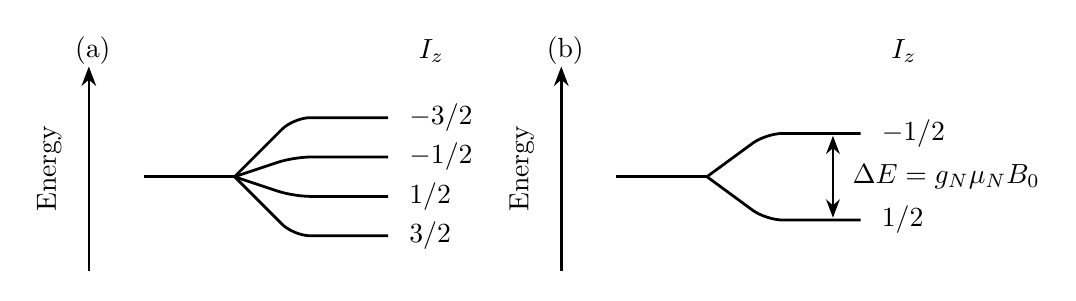
\begin{tikzpicture}[line width=0.8pt,>=Stealth]
% ---------- (a) I = 3/2 ----------
\begin{scope}
\node at (-0.15,3.05) {(a)};
\node at (4.15,3.05) {$I_z$};
% Energy 竖轴
\draw[->,line width=0.9] (-0.20,0.25) -- (-0.20,2.85);
\node[rotate=90,anchor=south] at (-0.42,1.55) {Energy};
% 未分裂能级 -> 四条等间距能级（最高为 -3/2）
\draw[line width=1.0] (0.50,1.45) -- (1.65,1.45);
\foreach \y in {2.20,1.70,1.20,0.70}{
  \draw[line width=1.0,rounded corners=6pt] (1.65,1.45) -- (2.40,\y) -- (3.60,\y);
}
\node[anchor=west] at (3.74,2.20) {$-3/2$};
\node[anchor=west] at (3.74,1.70) {$-1/2$};
\node[anchor=west] at (3.74,1.20) {$1/2$};
\node[anchor=west] at (3.74,0.70) {$3/2$};
\end{scope}
% ---------- (b) I = 1/2 ----------
\begin{scope}[shift={(6.0,0)}]
\node at (-0.15,3.05) {(b)};
\node at (4.15,3.05) {$I_z$};
\draw[->,line width=0.9] (-0.20,0.25) -- (-0.20,2.85);
\node[rotate=90,anchor=south] at (-0.42,1.55) {Energy};
\draw[line width=1.0] (0.50,1.45) -- (1.65,1.45);
\foreach \y in {2.00,0.90}{
  \draw[line width=1.0,rounded corners=6pt] (1.65,1.45) -- (2.40,\y) -- (3.60,\y);
}
\node[anchor=west] at (3.74,2.00) {$-1/2$};
\node[anchor=west] at (3.74,0.90) {$1/2$};
% 能级间距 ΔE
\draw[<->] (3.25,0.93) -- (3.25,1.97);
\node[anchor=west,inner sep=3pt] at (3.38,1.45) {$\Delta E = g_N \mu_N B_0$};
\end{scope}
\end{tikzpicture}
\end{document}
